The input values required for A.3.1 are shown below. Since the response equations use SI units, the listed values are converted before substitution. The projectile mass is denoted by \(m_p\) so that it remains distinct from the pendulum mass \(M\).

{ % do not increment counter
\begin{center}\small\begin{tabular}{@{}lll@{}}
\toprule\noalign{}
Quantity & Value & Unit \\
\midrule\noalign{}
\(g\) & 9.81 & \(\mathrm{m}/\mathrm{s}^{2}\) \\
\(L\) & 0.565 & m \\
\(M\) & 52.0 & kg \\
\(m_p\) & 0.0220 & kg \\
\(v_p\) & 945 & \(\mathrm{m}/\mathrm{s}\) \\
\(t_1\) & 10.0 & s \\
\(N_{\mathrm{osc}}\) & 10 & 1 \\
\bottomrule\end{tabular}\end{center}
}

For the pendulum, the small-angle restoring motion gives the undamped equation

\[\ddot{u}+\frac{g}{L}u=0.\]

Therefore, the natural frequency does not depend on the total mass, because the mass cancels from the ideal pendulum equation. The natural frequency and period are

\[\boxed{\omega_n=\sqrt{\frac{g}{L}}=4.16687\ \mathrm{rad}/\mathrm{s}}\qquad\text{(A.3.2)}\]

\[\boxed{\tau=\frac{2\pi}{\omega_n}=1.50789\ \mathrm{s}}\qquad\text{(A.3.2)}\]

During the short impact, the projectile embeds in the pendulum mass, so linear momentum is conserved. Since the pendulum mass starts at rest, the common velocity immediately after impact satisfies

\[m_pv_p+M(0)=(M+m_p)\dot{u}_0.\]

Solving for the initial velocity gives

\[\boxed{\dot{u}_0=\frac{m_pv_p}{M+m_p}=0.399639\ \mathrm{m}/\mathrm{s}}\qquad\text{(A.3.3)}\]

The pendulum is still vertical immediately after impact, so \(u_0=0\). Substitution into the undamped initial-value solution gives

\[u(t)=u_0\cos(\omega_nt)+\frac{\dot{u}_0}{\omega_n}\sin(\omega_nt).\]

Because \(u_0=0\), the response becomes

\[\boxed{u(t)=\frac{\dot{u}_0}{\omega_n}\sin(\omega_nt)=95.9085\sin(4.16687t)\ \mathrm{mm}}\qquad\text{(A.3.4)}\]

At \(t_1=10\ \mathrm{s}\), substitution into the response gives

\[\boxed{u(t_1)=95.9085\sin(4.16687\times10)\ \mathrm{mm}=-70.6461\ \mathrm{mm}}\qquad\text{(A.3.4)}\]

Ten oscillations span the interval

\[\boxed{t_{\mathrm{end}}=N_{\mathrm{osc}}\tau=10(1.50789)=15.0789\ \mathrm{s}}\qquad\text{(A.3.5)}\]

The response reaches its first positive maximum one quarter period after impact. The largest absolute response is therefore

\[\boxed{\left\lvert u\right\rvert_{\max}=\frac{\dot{u}_0}{\omega_n}=95.9085\ \mathrm{mm}}\qquad\text{(A.3.5.a)}\]

The ten-oscillation plot includes data tips at the first maximum and at \(t_1=10\ \mathrm{s}\). The plotted readings are

\[\boxed{u_{\max}=95.9\ \mathrm{mm}}\qquad\text{(A.3.5.a)}\]

\[\boxed{u(10\ \mathrm{s})=-70.6\ \mathrm{mm}}\qquad\text{(A.3.5.b)}\]

\begin{figure}[H]
\centering
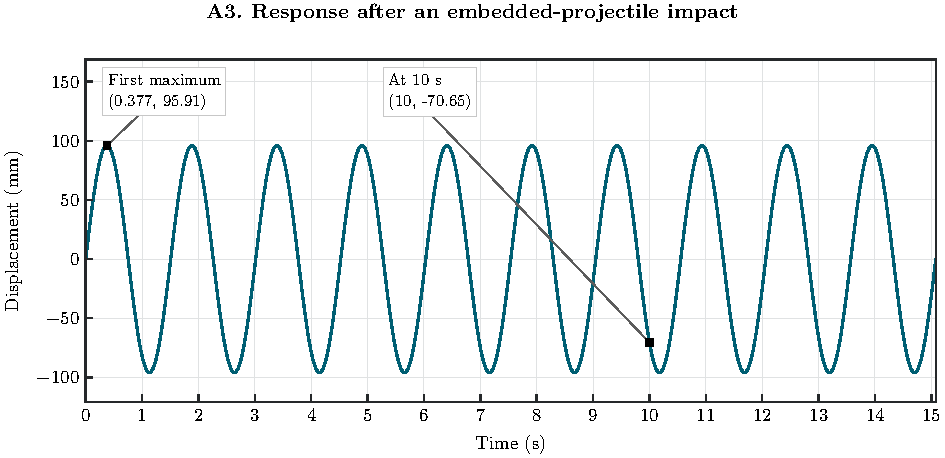
\includegraphics[width=0.95\linewidth,height=\textheight,keepaspectratio,alt={A.3.5.a-b. Linear pendulum response after impact with data tips at the first maximum and at ten seconds.}]{figures/generated/solutions/A3.pdf}
\caption{A.3.5.a-b. Impact response with data tips.}
\end{figure}

The projectile transfers its momentum to the combined mass, which produces a nonzero initial velocity but no initial displacement. The response consequently starts at zero, reaches its first maximum at \(t=\tau/4=0.377\ \mathrm{s}\), and then repeats with constant amplitude because damping is neglected. The maximum displacement corresponds to an angular amplitude of approximately \(u_{\max}/L=0.170\ \mathrm{rad}=9.73^{\circ}\), so the small-angle model is reasonable for this calculation. At \(10\ \mathrm{s}\), the pendulum is moving through the negative side of the motion rather than being at a maximum, which gives the plotted value of \(-70.6\ \mathrm{mm}\).

\clearpage
\thispagestyle{fancy}
\matlabcaption{Script used to plot the ten-oscillation response.}

\begin{center}
\begin{matlabcode}
g = 9.81;
L = 0.565;
M = 52;
mp = 0.022;
vp = 945;
t1 = 10;
Nosc = 10;
u0 = 0;

wn = sqrt(g/L);
tau = 2*pi/wn;
udot0 = mp*vp/(M+mp);
A = udot0/wn;

t = linspace(0,Nosc*tau,1000);
u = u0*cos(wn*t) + A*sin(wn*t);
u1 = u0*cos(wn*t1) + A*sin(wn*t1);

plot(t,1000*u,tau/4,1000*A,'ks',t1,1000*u1,'ks');
xlabel('Time (s)');
ylabel('u (mm)');
grid on;
\end{matlabcode}
\end{center}
\thispagestyle{fancy}
